\begin{statementbox}
\textbf{C091\quad 双曲线渐近线平行四边形面积定值}

设双曲线
\[
H:\ \frac{x^2}{a^2}-\frac{y^2}{b^2}=1,\qquad a>0,\ b>0,
\]
其两条渐近线为
\[
\ell_+:y=\frac ba x,\qquad \ell_-:y=-\frac ba x,
\]
交于 $O=(0,0)$。\textbf{任取} $P(x,y)\in H$，过 $P$ 分别作
$\ell_+$、$\ell_-$ 的平行线：前者交 $\ell_-$ 于 $R$，
后者交 $\ell_+$ 于 $Q$。四边形 $OQPR$ 是平行四边形。

\textbf{核心二级结论：}
\[
\boxed{\ S_{OQPR}=\frac{ab}{2}\ }.
\]
这是\textbf{与点 $P$ 的位置无关}的面积定值；$P$ 位于右支、左支、
上半部分或下半部分都成立。

\begin{center}
% C091 精确坐标示意图。取 a=3,b=2，H:x²/9-y²/4=1。
% P=(13/4,5/6) 在 H 上；Q=(9/4,3/2) 在 y=(2/3)x 上；
% R=(1,-2/3) 在 y=-(2/3)x 上；Q+R=P。
% 面积 |det(Q,R)|=3=ab/2。绝不自由近似修改点线关系。
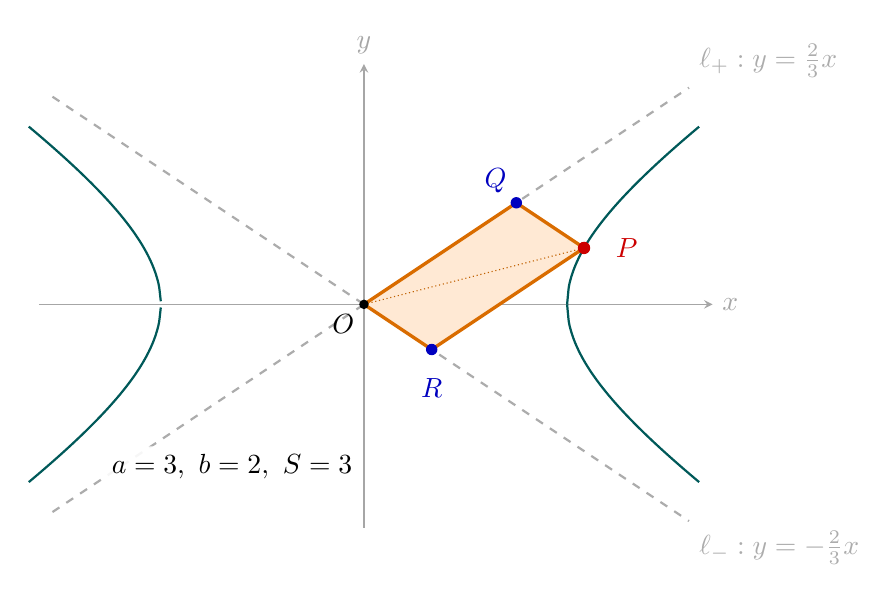
\begin{tikzpicture}[scale=0.86,>=stealth]
  \draw[->,gray!70] (-4.8,0)--(5.15,0) node[right] {$x$};
  \draw[->,gray!70] (0,-3.3)--(0,3.55) node[above] {$y$};
  \draw[gray!65,dashed,thick] (-4.6,-3.06667)--(4.8,3.2)
    node[above right] {$\ell_+:y=\frac23x$};
  \draw[gray!65,dashed,thick] (-4.6,3.06667)--(4.8,-3.2)
    node[below right] {$\ell_-:y=-\frac23x$};
  \draw[teal!70!black,thick,samples=80,domain=3:4.95,smooth]
    plot (\x,{(2/3)*sqrt(\x*\x-9)});
  \draw[teal!70!black,thick,samples=80,domain=3:4.95,smooth]
    plot (\x,{-(2/3)*sqrt(\x*\x-9)});
  \draw[teal!70!black,thick,samples=80,domain=-4.95:-3,smooth]
    plot (\x,{(2/3)*sqrt(\x*\x-9)});
  \draw[teal!70!black,thick,samples=80,domain=-4.95:-3,smooth]
    plot (\x,{-(2/3)*sqrt(\x*\x-9)});
  \coordinate (O) at (0,0);
  \coordinate (Q) at (2.25,1.5);
  \coordinate (R) at (1,-0.6666666667);
  \coordinate (P) at (3.25,0.8333333333);
  \fill[orange!17] (O)--(Q)--(P)--(R)--cycle;
  \draw[orange!85!black,very thick] (O)--(Q)--(P)--(R)--cycle;
  \draw[orange!75!black,densely dotted] (O)--(P);
  \fill (O) circle(2pt) node[below left] {$O$};
  \fill[blue!75!black] (Q) circle(2.4pt) node[above left] {$Q$};
  \fill[blue!75!black] (R) circle(2.4pt) node[below=7pt] {$R$};
  \fill[red!80!black] (P) circle(2.6pt) node[right=8pt] {$P$};
  \node[fill=white,fill opacity=.9,text opacity=1,rounded corners=2pt,
    inner sep=3pt] at (-1.95,-2.4) {$a=3,\ b=2,\ S=3$};
\end{tikzpicture}

\end{center}

\textbf{先用顶点猜结论（从特殊到一般）：}
取右顶点 $P=(a,0)$，直接得到
$Q=(a/2,b/2)$、$R=(a/2,-b/2)$。
此时 $QR=b$，$O$ 到直线 $QR$ 的距离为 $a/2$，
对角线 $QR$ 将四边形分成两个等面积三角形，因此
$S_{OQPR}=2\times\tfrac12\times b\times\tfrac a2=ab/2$。
\textbf{注意：}顶点只能用来\emph{猜测}定值；要证明任意点都成立，还需证明。

\textbf{读图约定：}一条边 $OQ$ 在 $\ell_+$ 上，另一条边 $OR$ 在 $\ell_-$ 上；
$P$ 与 $O$ 是\textbf{对顶点}，不是 $P$ 在渐近线上。
\textbf{识别信号：}“过双曲线上一点”“分别平行两条渐近线”
“所围四边形面积”“面积定值”。
\end{statementbox}

\clearpage
\begin{statementbox}
\textbf{更强的通式（任意平面点都能计算，双曲线时自动定值）。}

若 $P=(x,y)$ 是平面上任意一点，仍用同样的四条直线作平行四边形，则
\[
\boxed{\ S(P)=\frac{ab}{2}\left|\frac{x^2}{a^2}-\frac{y^2}{b^2}\right|\ }.
\]
\begin{itemize}
\item $P\in H$，括号内等于 $1$，故 $S=ab/2$；
\item 若 $x^2/a^2-y^2/b^2=t$，则 $S=\frac{ab}{2}|t|$；
\item 若 $P$ 位于任一渐近线上，则四边形退化，面积 $S=0$。
\end{itemize}
\textbf{定义边界：}若 $P$ 落在任一渐近线上，两组线的构造仍可进行，
但所得四边形\textbf{退化}，严格说不能称为非退化平行四边形；此时把面积定义为 $0$。

\textbf{特别说明：}面积相同\emph{不必然}推出 $P\in H$，
因为该通式带绝对值；例如 $P=(0,b)$ 不在 $H$ 上，却也得到 $S=ab/2$。
\end{statementbox}
